\phantomsection
\section*{Chapitre 3 : Pr\'evision et d\'etection d'anomalies dans le pilotage budg\'etaire}
\addcontentsline{toc}{section}{Chapitre 3 : Pr\'evision et d\'etection d'anomalies dans le pilotage budg\'etaire}

\bigskip

Le présent chapitre expose les fondements théoriques du dispositif de prévision budgétaire et de détection d'anomalies développé dans le cadre de ce mémoire. L'objectif n'est pas de présenter l'ensemble des méthodes existantes dans la littérature, mais de justifier les choix méthodologiques retenus au regard des caractéristiques du contexte étudié.

Le Ministère de la Justice gère un portefeuille composé de nombreuses lignes budgétaires aux comportements hétérogènes, dans un environnement marqué par des contraintes institutionnelles, opérationnelles et informationnelles spécifiques. La prévision de l'exécution budgétaire et l'identification des comportements atypiques constituent ainsi deux leviers complémentaires pour renforcer le pilotage des crédits et soutenir la prise de décision.

La première partie du chapitre présente les fondements de la prévision budgétaire, ses objectifs ainsi que les contraintes propres au secteur public. La deuxième partie est consacrée à la détection d'anomalies budgétaires et à son intérêt pour le suivi de l'exécution. La troisième partie justifie le choix des modèles de prévision retenus et décrit la méthode utilisée pour sélectionner le modèle le plus adapté à chaque ligne budgétaire. La quatrième partie présente les méthodes de détection d'anomalies mobilisées dans cette étude, à savoir le score Z et l'algorithme Isolation Forest. Enfin, la dernière partie expose les critères utilisés pour évaluer la qualité des prévisions produites.

Ce cadre théorique constitue la base de la démarche empirique mise en œuvre au chapitre suivant, où les méthodes retenues sont appliquées aux données budgétaires du Ministère de la Justice afin d'évaluer leur pertinence et leur apport au pilotage budgétaire.

%================================================================
\phantomsection
\subsection*{3.1 \quad Fondements de la pr\'evision budg\'etaire}
\addcontentsline{toc}{subsection}{3.1 Fondements de la pr\'evision budg\'etaire}
%================================================================

Apr\`es avoir pr\'esent\'e le cadre institutionnel du Minist\`ere de la
Justice ainsi que les m\'ecanismes de gestion et d'ex\'ecution budg\'etaire,
il convient d\'esormais de s'int\'eresser \`a la question de la pr\'evision.
En effet, la programmation budg\'etaire ne repose pas uniquement sur
l'analyse des d\'epenses pass\'ees~; elle implique \'egalement d'anticiper
l'\'evolution future des besoins et des niveaux d'ex\'ecution afin
d'\'eclairer la prise de d\'ecision.

Dans le contexte du secteur public, cet exercice pr\'esente des
particularit\'es importantes. Les cr\'edits sont r\'epartis entre de
nombreuses lignes budg\'etaires aux comportements parfois tr\`es
diff\'erents, tandis que les gestionnaires doivent composer avec des
contraintes r\'eglementaires, organisationnelles et op\'erationnelles
sp\'ecifiques. Produire une pr\'evision pertinente suppose donc de
comprendre \`a la fois la nature des donn\'ees disponibles, les objectifs
poursuivis par la pr\'evision et les limites inh\'erentes au contexte
\'etudi\'e.

Cette section pr\'esente ainsi les fondements de la pr\'evision
budg\'etaire, les contraintes propres au secteur public ainsi que les
principaux enjeux associ\'es \`a l'anticipation de l'ex\'ecution des
cr\'edits au sein du Minist\`ere de la Justice.

\subsubsection*{3.1.1 \quad D\'efinition et objectifs}
\addcontentsline{toc}{subsubsection}{3.1.1 \quad D\'efinition et objectifs}
La prévision budgétaire consiste à estimer l'évolution future d'une variable financière à partir des informations disponibles au moment de l'analyse. Elle vise à produire l'estimation la plus réaliste possible de l'avenir en s'appuyant sur les données historiques, la connaissance du contexte et les événements susceptibles d'influencer l'exécution future.

Dans le contexte du Ministère de la Justice, la prévision budgétaire constitue une étape essentielle du processus de programmation et de planification des crédits. Elle ne consiste pas à prévoir un montant global unique pour l'ensemble du ministère, mais à anticiper l'évolution de chacune des lignes budgétaires qui composent son budget.

Comprendre cet exercice suppose de rappeler brièvement la structure budgétaire présentée au chapitre précédent. Le budget du Ministère de la Justice se décompose en deux grandes catégories : les dépenses de fonctionnement, comprenant notamment les dépenses de personnel et les dépenses de matériel et dépenses diverses (MDD), et les dépenses d'investissement. Ces crédits sont ensuite répartis selon plusieurs niveaux d'organisation : programmes, projets, régions et, au niveau le plus détaillé, lignes budgétaires.

La ligne budgétaire constitue l'unité élémentaire d'exécution et représente l'objet central de cette étude. Elle correspond à une catégorie précise de dépense, telle que les frais de carburant, les indemnités ou les dépenses d'entretien. Chaque ligne possède son propre historique d'exécution et peut présenter un comportement différent de celui des autres lignes. Certaines évoluent de manière relativement stable au fil des années, tandis que d'autres connaissent des variations importantes liées à des événements ponctuels ou à des arbitrages budgétaires.

La prévision budgétaire doit donc tenir compte de cette hétérogénéité afin de produire des estimations pertinentes et directement exploitables pour la programmation triennale et le pilotage de l'exécution budgétaire. Dans ce travail, l'objectif n'est pas de prévoir le budget global du ministère, mais d'estimer l'évolution future de chaque ligne budgétaire afin de fournir une information plus fine et plus utile à la prise de décision.

La mise en place d'un dispositif de prévision budgétaire suppose d'abord de définir la variable à prévoir, l'horizon de prévision retenu ainsi que la fréquence de production des estimations.

Dans le cadre de cette étude, la variable retenue est le taux d'engagement annuel de chaque ligne budgétaire, défini comme le rapport entre le montant engagé et le crédit ouvert. Le montant engagé prévisionnel est ensuite obtenu par recomposition à partir du taux estimé et du crédit ouvert prévisionnel. Le choix de cette variable cible ainsi que la méthode de recomposition sont détaillés au chapitre 4.

L'horizon de prévision est déterminé par les besoins du processus budgétaire encadré par la LOF 130-13. Les prévisions doivent permettre d'alimenter à la fois la préparation du Projet de Loi de Finances (PLF) et la programmation budgétaire triennale. Le choix de l'horizon influence directement les méthodes mobilisées ainsi que le niveau d'incertitude associé aux estimations produites.

Les prévisions sont établies une fois par an, à la clôture de l'exercice N-1, afin d'éclairer la préparation de l'exercice N+1. Bien que cette fréquence soit relativement faible, elle justifie la mise en place d'un dispositif automatisé capable d'être réutilisé chaque année sur les nouvelles données d'exécution.

La construction d'un système de prévision nécessite également de prendre en compte l'usage qui sera fait des résultats produits. Les estimations générées ont vocation à alimenter la préparation budgétaire, à soutenir les arbitrages entre lignes, à renforcer le suivi de l'exécution et à faciliter l'analyse des écarts observés. Ces besoins influencent directement la forme des informations restituées aux gestionnaires.

Enfin, toute démarche de prévision repose sur la disponibilité de données fiables et exploitables. Dans le cas du Ministère de la Justice, l'analyse s'appuie sur l'historique des données d'exécution budgétaire disponibles pour les exercices étudiés. Une part importante du travail consiste à collecter, harmoniser et consolider ces données avant toute phase de modélisation.

L'ensemble de ces éléments constitue le socle sur lequel repose le dispositif développé dans ce mémoire. Leur mise en œuvre pratique est présentée au chapitre 4.

\bigskip

\subsubsection*{3.1.2 \quad Contraintes propres au contexte \'etudi\'e}
\addcontentsline{toc}{subsubsection}{3.1.2 \quad Contraintes propres au contexte \'etudi\'e}

La pr\'evision budg\'etaire dans le secteur public s'inscrit dans un contexte
particulier qui influence directement les m\'ethodes pouvant \^etre
mobilis\'ees. Dans le cadre de cette \'etude, trois contraintes principales
m\'eritent d'\^etre soulign\'ees.

La premi\`ere concerne la disponibilit\'e des donn\'ees. Les historiques
budg\'etaires exploitables restent relativement limit\'es \`a l'\'echelle de
chaque ligne budg\'etaire, ce qui r\'eduit la quantit\'e d'information
disponible pour l'apprentissage des mod\`eles de pr\'evision. Cette
caract\'eristique favorise le recours \`a des approches simples et robustes
plut\^ot qu'\`a des mod\`eles n\'ecessitant un volume important de donn\'ees.

La deuxi\`eme contrainte r\'eside dans l'h\'et\'erog\'en\'eit\'e des lignes
budg\'etaires. Certaines lignes pr\'esentent des comportements relativement
stables au fil des ann\'ees, tandis que d'autres connaissent des variations
plus marqu\'ees. Cette diversit\'e rend difficile l'utilisation d'un mod\`ele
unique pour l'ensemble du portefeuille budg\'etaire et justifie une approche
adapt\'ee aux caract\'eristiques de chaque ligne.

Enfin, l'ex\'ecution budg\'etaire est influenc\'ee par de nombreux facteurs
qui ne sont pas toujours observables dans les donn\'ees historiques. Les
arbitrages de gestion, les r\'eallocations de cr\'edits, les \'evolutions
r\'eglementaires ou encore certains \'ev\'enements exceptionnels peuvent
modifier le comportement d'une ligne budg\'etaire sans que ces changements
soient enti\`erement pr\'evisibles \`a partir du pass\'e. Les pr\'evisions
produites doivent donc \^etre interpr\'et\'ees comme des outils d'aide \`a la
d\'ecision et non comme des certitudes.

Ces contraintes ne constituent pas des obstacles \`a la pr\'evision, mais des
\'el\'ements de contexte qui orientent les choix m\'ethodologiques retenus
dans ce m\'emoire. Elles expliquent notamment le recours \`a des mod\`eles
adapt\'es aux s\'eries courtes ainsi qu'\`a un dispositif compl\'ementaire de
d\'etection d'anomalies.

\subsubsection*{3.1.3 \quad Enjeux de la pr\'evision budg\'etaire}
\addcontentsline{toc}{subsubsection}{3.1.3 \quad Enjeux de la pr\'evision budg\'etaire}

La pr\'evision budg\'etaire joue un r\^ole important dans le processus de
pr\'eparation, de programmation et de suivi des cr\'edits publics. En
fournissant une estimation de l'\'evolution future des lignes budg\'etaires,
elle permet d'\'eclairer les d\'ecisions prises lors de l'\'elaboration du
budget et de la programmation pluriannuelle.

Dans le contexte du Minist\`ere de la Justice, la pr\'evision contribue \`a
am\'eliorer la visibilit\'e sur les besoins futurs de financement et \`a
soutenir les arbitrages entre programmes, projets et r\'egions. Elle permet
\'egalement d'anticiper certaines situations de sous-ex\'ecution ou de
d\'epassement potentiel, offrant ainsi aux gestionnaires une information
compl\'ementaire pour le suivi de l'ex\'ecution budg\'etaire.

Au-del\`a de la production d'un chiffre pr\'evisionnel, l'enjeu r\'eside
dans la capacit\'e \`a fournir une information exploitable pour le pilotage.
Une pr\'evision utile doit \^etre accompagn\'ee d'\'el\'ements permettant
d'appr\'ecier son niveau de fiabilit\'e et d'identifier les situations
n\'ecessitant une attention particuli\`ere. C'est dans cette logique que le
dispositif propos\'e dans ce m\'emoire associe la pr\'evision budg\'etaire
\`a des indicateurs de fiabilit\'e et \`a un m\'ecanisme de d\'etection
d'anomalies, afin d'apporter aux gestionnaires des \'el\'ements d'analyse
compl\'ementaires \`a la simple estimation chiffr\'ee.

\subsubsection*{3.1.4 \quad Positionnement par rapport aux pratiques de pr\'evision budg\'etaire}
\addcontentsline{toc}{subsubsection}{3.1.4 \quad Positionnement par rapport aux pratiques de pr\'evision budg\'etaire}

La probl\'ematique trait\'ee dans ce m\'emoire ne concerne pas uniquement
le Minist\`ere de la Justice. La pr\'evision de l'ex\'ecution
budg\'etaire, le suivi des \'ecarts et l'am\'elioration de la qualit\'e
du reporting constituent des enjeux communs \`a l'ensemble des
administrations publiques. Les recommandations internationales en
mati\`ere de gestion des finances publiques insistent notamment sur la
n\'ecessit\'e de renforcer la pr\'evisibilit\'e de l'ex\'ecution
budg\'etaire, la qualit\'e du reporting financier et l'utilisation des
donn\'ees pour appuyer les d\'ecisions de gestion.

Dans cette perspective, le dispositif propos\'e ne pr\'etend pas
introduire une logique enti\`erement nouvelle. Il s'inscrit dans une
d\'emarche classique de pilotage budg\'etaire~: consolider les donn\'ees
disponibles, produire des projections, identifier les \'ecarts atypiques
et restituer les r\'esultats sous une forme exploitable par les
gestionnaires. Sa contribution r\'eside plut\^ot dans son adaptation au
contexte \'etudi\'e~: un historique annuel court, une granularit\'e par
ligne budg\'etaire, des contraintes de s\'ecurit\'e informatique et un
besoin op\'erationnel de simplicit\'e.

Ainsi, l'originalit\'e du travail ne r\'eside pas dans l'id\'ee
g\'en\'erale de pr\'evoir l'ex\'ecution budg\'etaire, d\'ej\`a pr\'esente
dans les pratiques de gestion publique, mais dans la construction d'un
dispositif l\'eger, local, reproductible et directement utilisable par
la Direction du Budget \`a partir des donn\'ees effectivement
disponibles.

%================================================================
\phantomsection
\subsection*{3.2 \quad Fondements de la d\'etection d'anomalies budg\'etaires}
\addcontentsline{toc}{subsection}{3.2 Fondements de la d\'etection d'anomalies budg\'etaires}
%================================================================

La d\'etection d'anomalies est un ensemble de m\'ethodes visant \`a identifier
des observations dont le comportement s'\'ecarte significativement de celui
attendu ou habituellement observ\'e. Son objectif est de mettre en \'evidence
des situations atypiques n\'ecessitant une analyse compl\'ementaire. Elle est
largement utilis\'ee dans de nombreux domaines tels que la finance
(d\'etection de fraudes), la cybers\'ecurit\'e (d\'etection d'intrusions),
l'industrie (maintenance pr\'edictive), la sant\'e (identification de valeurs
m\'edicales anormales) ou encore la gestion budg\'etaire, o\`u elle permet
de rep\'erer des comportements d'ex\'ecution inhabituels n\'ecessitant une
attention particuli\`ere.

Dans le contexte du Minist\`ere de la Justice, elle contribue \`a identifier
les lignes budg\'etaires dont l'ex\'ecution s'\'ecarte sensiblement des
tendances observ\'ees, afin d'orienter l'analyse des gestionnaires et de
renforcer le pilotage des cr\'edits. Toutefois, la d\'etection d'une anomalie
ne signifie pas n\'ecessairement l'existence d'un dysfonctionnement ou d'une
erreur de gestion. Dans de nombreux cas, ces \'ecarts r\'esultent de
d\'ecisions d\'elib\'er\'ees des gestionnaires, telles que des r\'eallocations
de ressources, des ajustements budg\'etaires en cours d'exercice ou la prise
en compte d'\'ev\'enements exceptionnels. Une anomalie doit donc \^etre
interpr\'et\'ee comme un signal d'attention n\'ecessitant une analyse
compl\'ementaire, et non comme la preuve d'un probl\`eme.

Dans le cadre de cette \'etude, plusieurs m\'ethodes de d\'etection d'anomalies
ont \'et\'e examin\'ees afin d'identifier celles qui r\'epondaient le mieux aux
caract\'eristiques des donn\'ees budg\'etaires analys\'ees. Cette d\'emarche a
conduit \`a la conception d'un dispositif combinant deux approches
compl\'ementaires~: le \textbf{score~Z}, destin\'e \`a rep\'erer les anomalies
ponctuelles au sein d'une ligne budg\'etaire, et l'\textbf{Isolation Forest},
utilis\'ee pour d\'etecter les lignes pr\'esentant un comportement globalement
atypique. L'association de ces deux m\'ethodes permet d'obtenir une d\'etection
plus compl\`ete et plus pertinente qu'une utilisation isol\'ee de chacune
d'elles.

\subsubsection*{3.2.1 \quad D\'efinition et typologie des anomalies}
\addcontentsline{toc}{subsubsection}{3.2.1 \quad D\'efinition et typologie des anomalies}

Une \textbf{anomalie budg\'etaire}, au sens retenu ici, est une observation
d'ex\'ecution qui s'\'ecarte sensiblement du comportement attendu d'une ligne,
soit par rapport \`a son propre historique, soit par rapport \`a l'ensemble du
portefeuille. La d\'efinition est volontairement statistique et neutre~: elle
ne porte aucun jugement sur les causes de l'\'ecart, qui peuvent rel\`ever
d'\'ev\'enements exog\`enes l\'egitimes (virements, ouvertures de cr\'edits,
d\'ecisions de programmation) tout autant que d'al\'eas d'ex\'ecution. Une
anomalie est un signal qui m\'erite v\'erification, et non un verdict.

Plut\^ot que d'adopter une typologie purement th\'eorique
(anomalie~ponctuelle, anomalie~de~ligne, anomalie~collective), nous retenons
une grille \textbf{op\'erationnelle}, directement align\'ee sur les
cat\'egories effectivement produites par le dispositif final et restitu\'ees
au gestionnaire dans le tableau de bord. \`A chaque classe correspond un
niveau d'urgence, qui guide l'attention du gestionnaire.

\textbf{(a) Anomalie r\'ecente:} \'Ecart significatif observ\'e sur l'exercice
le plus r\'ecent par rapport \`a l'historique propre de la ligne -- par
exemple un taux d'engagement \`a 145\,\% en 2025 sur une ligne dont la
moyenne historique est de 90\,\%. Cette anomalie est d\'etect\'ee
principalement par le \textbf{score~Z} appliqu\'e ligne par ligne et ann\'ee
par ann\'ee, et appelle une attention \'elev\'ee.

\textbf{(b) Anomalie structurelle:} Ligne pr\'esentant un profil
d'ex\'ecution atypique sur plusieurs ann\'ees au regard de l'ensemble du
portefeuille -- par exemple un taux qui oscille entre 30\,\% et 200\,\% alors
que la majorit\'e des lignes se situent entre 80\,\% et 100\,\%. Cette
anomalie suppose une comparaison des profils entre eux et est d\'etect\'ee
principalement par l'\textbf{Isolation Forest}~; elle appelle une vigilance
mod\'er\'ee mais r\'eguli\`ere.

\textbf{(c) Anomalie critique:} Combinaison d'une anomalie r\'ecente et
d'un profil structurellement atypique sur la m\^eme ligne. Cette
configuration -- la ligne s'\'ecarte \`a la fois de son propre historique
\emph{et} du comportement g\'en\'eral du portefeuille -- est la plus urgente
de toutes et n\'ecessite une intervention prioritaire du gestionnaire.

\textbf{(d) Surconsommation structurelle:} Taux d'engagement durablement
sup\'erieur au niveau habituel (taux moyen $>$ 100\,\%), sans \'ecart r\'ecent
au sens du score~Z. Cette configuration peut r\'ev\'eler un besoin r\'ecurrent
de r\'eallocation des cr\'edits plut\^ot qu'une d\'erive ponctuelle, et appelle
une vigilance mod\'er\'ee.

\textbf{(e) Comportement normal:} Absence de signal significatif sur les deux
d\'etecteurs. Aucune action particuli\`ere n'est requise au-del\`a du suivi
ordinaire.

Cette typologie n'est pas une simple cat\'egorisation~: elle conditionne le
choix m\'ethodologique de la section~3.4. Le dispositif final associe un
d\'etecteur \og ann\'ee \fg{} (score~Z, qui rep\`ere les anomalies r\'ecentes)
et un d\'etecteur \og ligne \fg{} (Isolation Forest, qui rep\`ere les
anomalies structurelles), puis croise les deux signaux pour produire les
niveaux de priorit\'e op\'erationnelle restitu\'es au gestionnaire. Ignorer
l'un des deux d\'etecteurs reviendrait \`a passer \`a c\^ot\'e d'une
cat\'egorie enti\`ere d'anomalies.

\subsubsection*{3.2.2 \quad Int\'er\^et pour le pilotage budg\'etaire}
\addcontentsline{toc}{subsubsection}{3.2.2 \quad Int\'er\^et pour le pilotage budg\'etaire}

La d\'etection d'anomalies contribue \`a am\'eliorer le pilotage budg\'etaire en
orientant l'attention des gestionnaires vers les situations les plus
susceptibles de n\'ecessiter une analyse approfondie. Dans un contexte o\`u
plusieurs centaines de lignes budg\'etaires doivent \^etre suivies
simultan\'ement, il est difficile d'examiner chacune d'entre elles avec le
m\^eme niveau de d\'etail.

Un dispositif de d\'etection permet ainsi d'identifier les lignes dont le
comportement s'\'ecarte significativement des habitudes observ\'ees ou des
pr\'evisions \'etablies. \`A la cl\^oture d'un exercice, il facilite l'analyse
des \'ecarts d'ex\'ecution. En cours d'ann\'ee, il contribue \`a rep\'erer les
d\'erives \'emergentes et \`a renforcer la vigilance des gestionnaires. Lors
de la pr\'eparation budg\'etaire, il aide \'egalement \`a cibler les lignes
n\'ecessitant un examen particulier ou une r\'e\'evaluation des hypoth\`eses
retenues.

L'objectif n'est pas de remplacer le jugement du gestionnaire mais de le
soutenir. En r\'eduisant le nombre de lignes n\'ecessitant une attention
prioritaire, la d\'etection d'anomalies permet de concentrer les efforts
d'analyse sur les situations pr\'esentant le risque le plus \'elev\'e.

\subsubsection*{3.2.3 \quad Apports \`a l'aide \`a la d\'ecision}
\addcontentsline{toc}{subsubsection}{3.2.3 \quad Apports \`a l'aide \`a la d\'ecision}

La d\'etection d'anomalies ne remplace pas le jugement du gestionnaire et ne
conduit pas automatiquement \`a une action corrective. Une anomalie signale
simplement qu'un comportement m\'erite une analyse plus approfondie. Dans de
nombreux cas, l'\'ecart observ\'e r\'esulte d'une d\'ecision de gestion
parfaitement justifi\'ee ou d'un \'ev\'enement exceptionnel connu des
responsables budg\'etaires.

Son principal apport r\'eside donc dans l'aide \`a la d\'ecision. En mettant
en \'evidence les lignes pr\'esentant les comportements les plus atypiques, le
dispositif facilite l'analyse des donn\'ees et permet aux gestionnaires de
concentrer leur attention sur un nombre limit\'e de situations potentiellement
importantes. Il contribue ainsi \`a structurer l'examen des lignes
budg\'etaires, \`a documenter les \'echanges entre acteurs et \`a orienter les
investigations lorsque cela est n\'ecessaire.

La valeur du dispositif ne r\'eside donc pas dans la production d'une
d\'ecision automatique, mais dans sa capacit\'e \`a fournir aux gestionnaires
des \'el\'ements d'information suppl\'ementaires pour \'eclairer leur jugement.

%================================================================
\phantomsection
\subsection*{3.3 \quad Mod\`eles de pr\'evision adapt\'es aux s\'eries budg\'etaires courtes}
\addcontentsline{toc}{subsection}{3.3 Mod\`eles de pr\'evision adapt\'es aux s\'eries budg\'etaires courtes}
%================================================================

\subsubsection*{3.3.1 \quad Justification du choix des mod\`eles retenus}
\addcontentsline{toc}{subsubsection}{3.3.1 \quad Justification du choix des mod\`eles retenus}

Le choix des mod\`eles retenus est directement li\'e aux caract\'eristiques des
donn\'ees disponibles. Au niveau de chaque ligne budg\'etaire, l'historique
exploitable se limite \`a cinq observations annuelles, ce qui constitue un
volume d'information particuli\`erement r\'eduit pour l'estimation de mod\`eles
complexes.

Une phase exploratoire a n\'eanmoins permis d'\'evaluer plusieurs approches de
pr\'evision plus sophistiqu\'ees, notamment la r\'egression Ridge, la r\'egression
Lasso et le gradient boosting (XGBoost) \citep{Hastie2009, Chen2016}. Les
r\'esultats obtenus se sont r\'ev\'el\'es peu satisfaisants dans le contexte
\'etudi\'e, avec des erreurs de pr\'evision plus \'elev\'ees et une faible
stabilit\'e des estimations d'une ligne \`a l'autre. Ces m\'ethodes
n\'ecessitent g\'en\'eralement un volume de donn\'ees plus important pour
exprimer pleinement leur potentiel.

Compte tenu de ces contraintes, le choix s'est orient\'e vers des mod\`eles plus
simples et plus robustes face \`a la raret\'e des donn\'ees. Cinq approches ont
ainsi \'et\'e retenues~: la tendance lin\'eaire, la moyenne historique, la
moyenne pond\'er\'ee, la persistance (na\"ive) et le lissage exponentiel
simple \citep{Hyndman2021, Makridakis2018}. Ces mod\`eles pr\'esentent
l'avantage d'\^etre interpr\'etables, faciles \`a mettre en \oe{}uvre et
adapt\'es \`a des s\'eries temporelles courtes.

Le choix retenu ne vise donc pas \`a identifier le mod\`ele le plus
sophistiqu\'e, mais le mod\`ele le plus adapt\'e aux caract\'eristiques des
donn\'ees disponibles et aux besoins op\'erationnels du Minist\`ere de la
Justice.

\subsubsection*{3.3.2 \quad Les cinq mod\`eles de pr\'evision retenus}
\addcontentsline{toc}{subsubsection}{3.3.2 \quad Les cinq mod\`eles de pr\'evision retenus}

Les cinq mod\`eles retenus sont appliqu\'es au taux d'engagement annuel de
chaque ligne budg\'etaire. Le choix de cette variable permet de travailler sur
une mesure plus stable que le montant engag\'e brut, tout en conservant une
interpr\'etation directement li\'ee \`a l'ex\'ecution budg\'etaire.

\textbf{La tendance lin\'eaire} repose sur l'hypoth\`ese qu'une \'evolution
observ\'ee dans le pass\'e se poursuivra selon une tendance similaire dans le
futur. Elle est particuli\`erement adapt\'ee aux lignes pr\'esentant une
progression ou une diminution relativement r\'eguli\`ere au fil des ann\'ees.
Les coefficients $a$ et $b$ sont estim\'es par moindres carr\'es ordinaires sur
l'historique disponible, puis appliqu\'es \`a l'ann\'ee cible~:
$$
\widehat{x}_{Y+1} \;=\; a \cdot (Y+1) + b,
\qquad
(a,b) = \arg\min_{a,b} \sum_{y=1}^{n} \bigl(x_y - a y - b\bigr)^2.
$$

\textbf{La moyenne historique} consiste \`a utiliser la moyenne des taux
d'engagement observ\'es sur l'historique disponible. Cette approche convient
aux lignes dont le comportement est globalement stable et ne pr\'esente pas
de tendance marqu\'ee.
$$
\overline{x} \;=\; \frac{1}{n} \sum_{y=1}^{n} x_y,
\qquad
\widehat{x}_{Y+1} \;=\; \overline{x}.
$$

\textbf{La moyenne pond\'er\'ee} attribue davantage d'importance aux
observations r\'ecentes qu'aux observations plus anciennes. Elle permet ainsi
de prendre en compte d'\'eventuels changements r\'ecents dans le comportement
d'une ligne budg\'etaire. Les poids cro\^issent lin\'eairement avec l'anciennet\'e
inverse de l'observation~:
$$
\widehat{x}_{Y+1} \;=\; \sum_{y=1}^{n} w_y \, x_y,
\qquad
w_y = \frac{y}{\sum_{k=1}^{n} k} = \frac{2y}{n(n+1)}.
$$

\textbf{La persistance (mod\`ele na\"if)} suppose que le comportement observ\'e
lors du dernier exercice se reproduira \`a l'exercice suivant. Malgr\'e sa
simplicit\'e, ce mod\`ele constitue souvent une r\'ef\'erence pertinente pour
\'evaluer la performance des autres approches.
$$
\widehat{x}_{Y+1} \;=\; x_Y .
$$

\textbf{Le lissage exponentiel simple} repr\'esente un compromis entre la
moyenne historique et la persistance. Il accorde davantage de poids aux
observations r\'ecentes tout en conservant l'information contenue dans
l'ensemble de l'historique disponible. La pr\'evision suit la r\'ecurrence~:
$$
\widehat{x}_{y+1} \;=\; \alpha\, x_y + (1-\alpha)\, \widehat{x}_y,
\qquad \alpha \in [0,1],
$$
o\`u le param\`etre de lissage $\alpha$ est optimis\'e automatiquement par
maximum de vraisemblance sur l'historique de chaque ligne. Une valeur de
$\alpha$ proche de~1 rapproche le mod\`ele de la persistance, tandis qu'une
valeur proche de~0 le rapproche de la moyenne historique.

Ces cinq mod\`eles couvrent ainsi diff\'erents comportements possibles des
lignes budg\'etaires~: tendance progressive, stabilit\'e autour d'une moyenne,
prise en compte des \'evolutions r\'ecentes ou prolongement du comportement
le plus r\'ecent. La section suivante pr\'esente la m\'ethode retenue pour
s\'electionner le mod\`ele le plus adapt\'e \`a chaque ligne budg\'etaire.

\subsubsection*{3.3.3 \quad S\'election du mod\`ele par ligne budg\'etaire}
\addcontentsline{toc}{subsubsection}{3.3.3 \quad S\'election du mod\`ele par ligne budg\'etaire}

Les lignes budg\'etaires du Minist\`ere de la Justice pr\'esentent des
comportements tr\`es diff\'erents. Certaines \'evoluent de mani\`ere relativement
r\'eguli\`ere d'une ann\'ee \`a l'autre, tandis que d'autres connaissent des
variations importantes li\'ees \`a des \'ev\'enements ponctuels, \`a des
arbitrages budg\'etaires ou \`a la nature m\^eme de la d\'epense concern\'ee.
Dans ce contexte, l'utilisation d'un mod\`ele unique pour l'ensemble des
lignes appara\^it peu adapt\'ee.

La d\'emarche retenue consiste donc \`a comparer les cinq mod\`eles de
pr\'evision pr\'ec\'edemment pr\'esent\'es pour chaque ligne budg\'etaire.
L'objectif n'est pas d'identifier un mod\`ele universellement sup\'erieur aux
autres, mais de d\'eterminer celui qui reproduit le mieux le comportement
historique de la ligne consid\'er\'ee.

Pour cela, les performances de chaque mod\`ele sont \'evalu\'ees \`a partir des
ann\'ees disponibles, en comparant les pr\'evisions obtenues aux valeurs
r\'eellement observ\'ees. Pour chaque ligne, le mod\`ele pr\'esentant le MAPE
moyen le plus faible est retenu comme mod\`ele de r\'ef\'erence.

Cette approche pr\'esente deux avantages principaux. D'une part, elle tient
compte de l'h\'et\'erog\'en\'eit\'e des comportements budg\'etaires en adaptant le
mod\`ele \`a chaque ligne plut\^ot qu'en imposant une m\'ethode unique \`a
l'ensemble du portefeuille. D'autre part, elle permet d'associer \`a chaque
pr\'evision un indicateur objectif de fiabilit\'e fond\'e sur les performances
pass\'ees du mod\`ele retenu.

Ainsi, la pr\'evision finale ne r\'esulte pas du choix \textit{a priori} d'une
m\'ethode particuli\`ere, mais d'un processus de s\'election fond\'e sur les
r\'esultats observ\'es sur les donn\'ees historiques de chaque ligne
budg\'etaire.

%================================================================
% --- ANCIENNES SOUS-SECTIONS 3.3.1--3.3.4 SUPPRIM\'EES ---
% Le contenu ci-dessous a \'et\'e remplac\'e par les trois nouvelles
% sous-sections 3.3.1--3.3.3. Section conserv\'ee comment\'ee pour r\'ef\'erence.
%================================================================
\iffalse
\subsubsection*{Anc. 3.3.1 \quad Limites des approches riches en param\`etres}

La litt\'erature r\'ecente en pr\'evision financi\`ere accorde une place
croissante aux m\'ethodes dites \og riches en param\`etres \fg{}~: r\'egressions
Lasso et Ridge, for\^ets al\'eatoires, gradient boosting (XGBoost, LightGBM),
r\'eseaux de neurones. Plusieurs travaux cit\'es au chapitre~2 montrent qu'elles
am\'eliorent la pr\'ecision sur des s\'eries longues et multivari\'ees. La
tentation est grande de les transposer au contexte budg\'etaire marocain.

Cette transposition est ici \emph{contre-indiqu\'ee}, pour deux raisons
convergentes.

La premi\`ere raison est d'ordre \textbf{statistique}. Ces m\'ethodes supposent
un nombre d'observations $n$ tr\`es sup\'erieur au nombre de param\`etres
effectifs $p$. Au niveau \og programme--projet--ligne \fg{}, nous disposons de
$n=5$ ann\'ees observ\'ees (2021--2025), et m\^eme $n=4$ pour la phase
d'entra\^inement la plus longue de la validation. Un mod\`ele Ridge avec
quatre r\'egresseurs saturerait d\'ej\`a la condition $n>p$~; un XGBoost
m\^eme l\'eg\`erement param\'etr\'e serait en situation de sur-apprentissage~:
il interpolerait les quatre points d'entra\^inement au prix d'une variance
hors-\'echantillon \'elev\'ee. Cet argument n'est pas seulement th\'eorique~:
une exp\'erimentation pr\'eliminaire, document\'ee au chapitre~4, montre qu'un
Lasso r\'egularis\'e produit sur les 321~lignes un MAPE de validation
sup\'erieur de 40\,\% \`a celui d'une simple tendance lin\'eaire OLS, avec en
outre des pr\'evisions occasionnellement n\'egatives sur des engagements
n\'ecessairement positifs.

La seconde raison rel\`eve de \textbf{l'usage institutionnel des r\'esultats}.
Les gestionnaires budg\'etaires attendent une m\'ethode dont chaque pr\'evision
puisse \^etre reconstruite \`a la main et expliqu\'ee en quelques lignes. Un
gradient boosting fournirait certes un chiffre, mais pas de justification
transparente. Dans le contexte \'etudi\'e, ce d\'eficit d'interpr\'etabilit\'e
constitue une limite suppl\'ementaire \`a leur utilisation.

Le choix de la parcimonie n'est donc ni un repli prudent ni un refus de la
modernit\'e statistique~: c'est l'application du principe selon lequel la
complexit\'e d'un mod\`ele doit \^etre adapt\'ee \`a l'information r\'eellement
disponible et aux contraintes d'usage du r\'esultat.

\subsubsection*{3.3.2 \quad Le compromis biais-variance en r\'egime de donn\'ees rares}
\addcontentsline{toc}{subsubsection}{3.3.2 \quad Le compromis biais-variance en r\'egime de donn\'ees rares}

Toute m\'ethode de pr\'evision peut \^etre analys\'ee \`a travers la
d\'ecomposition classique de l'erreur quadratique moyenne~:
$$
\mathrm{EQM}(\hat{y}) \;=\; \underbrace{\bigl[\mathbb{E}(\hat{y}) - y\bigr]^2}_{\text{biais}^2}
\;+\; \underbrace{\mathbb{V}(\hat{y})}_{\text{variance}}
\;+\; \underbrace{\sigma_\varepsilon^2}_{\text{bruit irr\'eductible}}.
$$
Le \textbf{biais} mesure l'\'ecart syst\'ematique entre la pr\'evision moyenne
et la vraie valeur~; il p\'enalise les mod\`eles trop rigides, incapables de
capter la structure du ph\'enom\`ene. La \textbf{variance} mesure la
sensibilit\'e du mod\`ele aux fluctuations de l'\'echantillon
d'apprentissage~; elle p\'enalise les mod\`eles trop flexibles, qui
surr\'eagissent au bruit. Le \textbf{bruit irr\'eductible} est, par
d\'efinition, hors de port\'ee de toute m\'ethode.

Lorsque les donn\'ees sont abondantes, un mod\`ele flexible bien
r\'egularis\'e peut obtenir un biais faible et une variance ma\^itris\'ee.
Lorsque les donn\'ees sont rares ($n=5$), c'est m\'ecaniquement impossible~:
chaque param\`etre suppl\'ementaire est estim\'e \`a partir de tr\`es peu
d'observations et la variance de l'estim\'e augmente fortement. La
strat\'egie raisonnable consiste alors \`a accepter un biais l\'eg\`erement
plus \'elev\'e en \'echange d'une variance fortement r\'eduite, en privil\'egiant
des mod\`eles \`a peu de param\`etres dont le comportement hors-\'echantillon
est plus stable.

C'est cette logique qui pr\'eside au choix des cinq mod\`eles d\'ecrits
ci-apr\`es. Aucun ne d\'epasse \textbf{deux param\`etres effectifs}~: le plus
complexe (tendance lin\'eaire) en utilise deux, les autres un seul ou
z\'ero. Cette parcimonie n'est pas un appauvrissement~: c'est la r\'eponse
adapt\'ee \`a l'information statistique r\'eellement disponible.

\subsubsection*{3.3.3 \quad Les cinq mod\`eles parcimonieux retenus}
\addcontentsline{toc}{subsubsection}{3.3.3 \quad Les cinq mod\`eles parcimonieux retenus}

Une d\'ecision m\'ethodologique pr\'ealable conditionne tous les choix qui
suivent~: les cinq mod\`eles sont appliqu\'es non au montant brut engag\'e
mais au \textbf{taux d'engagement annuel}~:
$$
\tau_y \;=\; \frac{\mathrm{Engag\acute{e}}_y}{\mathrm{CO}_y}.
$$
La pr\'evision du montant est ensuite obtenue par recomposition~:
$\widehat{\mathrm{Engag\acute{e}}}_{N+1} = \widehat{\mathrm{CO}}_{N+1} \times \widehat{\tau}_{N+1}$.
Deux raisons motivent ce choix. D'une part, le taux est born\'e (typiquement
entre 0 et 1{,}3) et donc beaucoup plus stable dans le temps que le montant
brut. D'autre part, il s\'epare proprement la part \og enveloppe \fg{}
(politique, vot\'ee) de la part \og consommation \fg{} (op\'erationnelle,
observ\'ee).

Les cinq mod\`eles retenus, tous appliqu\'es au taux, sont les suivants.

\textbf{(1) Tendance lin\'eaire OLS.} On ajuste $\tau_y = a \cdot y + b$ par
moindres carr\'es sur l'historique. Pr\'evision~:
$\widehat{\tau}_{N+1} = a(N+1)+b$. Deux param\`etres. Pertinent pour les
lignes qui suivent une trajectoire monotone (croissance progressive d'un
poste de personnel par exemple).

\textbf{(2) Moyenne historique simple.} $\widehat{\tau}_{N+1} = \bar{\tau}$.
Un param\`etre. Adapt\'e aux lignes qui oscillent autour d'une valeur stable
sans tendance marqu\'ee (charges r\'ecurrentes du si\`ege).

\textbf{(3) Moyenne pond\'er\'ee r\'ecente.}
$\widehat{\tau}_{N+1} = \sum w_y \tau_y$ avec poids croissants
$w_y \propto y$ (par exemple $1, 2, 3, 4, 5$ pour les cinq ann\'ees). Un
param\`etre effectif (la s\'equence de poids est fix\'ee). Donne plus de
poids aux derniers exercices~; pertinent lorsqu'un changement de r\'egime
r\'ecent est suspect\'e mais non encore confirm\'e.

\textbf{(4) Persistance (mod\`ele na\"if).} $\widehat{\tau}_{N+1} = \tau_N$.
Z\'ero param\`etre estim\'e. Sert de r\'ef\'erence statistique~: aucune
m\'ethode plus sophistiqu\'ee ne peut \^etre justifi\'ee si elle n'am\'eliore
pas la persistance. Souvent meilleure que la moyenne pour les lignes
stationnaires r\'ecemment perturb\'ees.

\textbf{(5) Lissage exponentiel simple (SES).}
$\widehat{\tau}_{N+1} = \alpha \tau_N + (1-\alpha) \widehat{\tau}_N$, avec
$\alpha = 0{,}5$ fix\'e. Un param\`etre effectif, choisi \textit{a priori}
pour \'eviter une optimisation hasardeuse sur $n=5$. Compromis entre
persistance pure et moyenne historique~; utile pour les lignes qui pr\'esentent
une certaine inertie sans tendance claire.

L'ensemble couvre donc trois r\'egimes diff\'erents~: tendance (mod\`ele~1),
niveau moyen (2,~3,~5) et mouvement r\'ecent (4,~5). Cette diversit\'e
justifie l'\'etape de s\'election par ligne d\'ecrite \`a la sous-section
suivante.

\subsubsection*{3.3.4 \quad S\'election par ligne : reconna\^itre l'h\'et\'erog\'en\'eit\'e des comportements}
\addcontentsline{toc}{subsubsection}{3.3.4 \quad S\'election par ligne : reconna\^itre l'h\'et\'erog\'en\'eit\'e des comportements}

Les 321~lignes du portefeuille pr\'esentent des comportements tr\`es
diff\'erents~: certaines suivent une trajectoire quasi lin\'eaire (postes de
personnel), d'autres oscillent autour d'une moyenne (charges courantes du
si\`ege), d'autres encore subissent des chocs ponctuels (frais de justice
li\'es \`a un proc\`es exceptionnel). Imposer un mod\`ele unique \`a
l'ensemble du portefeuille serait peu justifi\'e th\'eoriquement et
contre-productif en pratique.

La strat\'egie retenue consiste \`a \textbf{s\'electionner le meilleur des
cinq mod\`eles ligne par ligne}, sur la base d'un \textbf{backtest \`a
horizon glissant}. Pour chaque ann\'ee de validation
$y \in \{2023, 2024, 2025\}$, on entra\^ine les cinq mod\`eles sur les
exercices ant\'erieurs \`a $y$, on pr\'edit $\widehat{\tau}_y$, on calcule le
MAPE de chaque mod\`ele par rapport au taux r\'eellement observ\'e, et on
retient pour la ligne le mod\`ele dont le MAPE moyen sur les trois ann\'ees
de validation est le plus faible. Le m\^eme mod\`ele est ensuite r\'eappliqu\'e,
entra\^in\'e cette fois sur toutes les ann\'ees disponibles, pour produire la
pr\'evision officielle de $N+1$.

Cette logique pr\'esente deux avantages. D'une part, le mod\`ele retenu pour
chaque ligne est empiriquement justifi\'e sur cette ligne~: si la tendance
lin\'eaire l'emporte sur la persistance, c'est qu'elle a effectivement mieux
pr\'edit le pass\'e. D'autre part, le MAPE de validation devient un indicateur
de la \textbf{fiabilit\'e} du couple mod\`ele-ligne, exploit\'e en
sous-section~3.5.2 pour produire un label \og Confiance Globale \fg{} transmis
au gestionnaire avec chaque pr\'evision.

La r\'epartition empirique des cinq mod\`eles sur les 321~lignes,
document\'ee au chapitre~4, confirme cette h\'et\'erog\'en\'eit\'e~: aucun
mod\`ele ne d\'epasse 50\,\% de parts du portefeuille~; chacun trouve sa
pertinence sur un sous-ensemble sp\'ecifique des lignes.
\fi

%================================================================
\phantomsection
\subsection*{3.4 \quad M\'ethodes de d\'etection d'anomalies retenues}
\addcontentsline{toc}{subsection}{3.4 M\'ethodes de d\'etection d'anomalies retenues}
%================================================================

\subsubsection*{3.4.1 \quad Le score Z appliqu\'e au taux d'engagement annuel}
\addcontentsline{toc}{subsubsection}{3.4.1 \quad Le score Z appliqu\'e au taux d'engagement annuel}

Le \textbf{score~Z} est le plus simple des d\'etecteurs d'anomalies
univari\'es. Pour chaque ligne $\ell$ et chaque ann\'ee $y$, on calcule~:
$$
z_{\ell,y} \;=\; \frac{\tau_{\ell,y} - \bar{\tau}_\ell}{\sigma_\ell},
$$
o\`u $\bar{\tau}_\ell$ et $\sigma_\ell$ d\'esignent la moyenne et l'\'ecart-type
du taux d'engagement de la ligne sur l'ensemble de son historique. Une ann\'ee
est consid\'er\'ee comme anormale au sens du Z d\`es lors que
$|z_{\ell,y}| > 1{,}5$.

Le seuil de \textbf{$\pm 1{,}5\sigma$} m\'erite une br\`eve justification.
Dans la litt\'erature, le seuil de $\pm 2\sigma$ est souvent retenu pour
identifier les observations atypiques. Toutefois, ce choix est principalement
adapt\'e \`a des s\'eries disposant d'un nombre suffisant d'observations.
Dans le cadre de cette \'etude, chaque ligne budg\'etaire ne dispose que de
cinq ann\'ees d'historique, ce qui rend l'estimation de la moyenne et de
l'\'ecart-type particuli\`erement sensible aux variations observ\'ees.

Afin d'adapter la m\'ethode \`a cette contrainte, plusieurs seuils ont \'et\'e
test\'es sur l'historique disponible. Un seuil de $\pm 2\sigma$ s'est r\'ev\'el\'e
trop restrictif, laissant passer certains \'ecarts pourtant significatifs au
regard de l'\'evolution des lignes budg\'etaires. \`A l'inverse, des seuils
plus faibles g\'en\'eraient un nombre important d'alertes, r\'eduisant la
lisibilit\'e des r\'esultats et augmentant la charge d'analyse pour les
gestionnaires.

Le seuil de $\pm 1{,}5\sigma$ a finalement \'et\'e retenu car il offre un
compromis satisfaisant entre sensibilit\'e et s\'electivit\'e. Il permet de
d\'etecter les \'ecarts les plus pertinents tout en maintenant un volume
d'alertes compatible avec une analyse op\'erationnelle. Les anomalies ainsi
identifi\'ees sont ensuite compl\'et\'ees par l'Isolation Forest, qui apporte
un second niveau d'analyse et de priorisation des lignes \`a examiner.

Les hypoth\`eses sous-jacentes sont assum\'ees~: la m\'ethode suppose
implicitement une distribution sym\'etrique autour de la moyenne, ce qui
n'est pas exactement le cas du taux d'engagement (born\'e par 0 \`a gauche,
par 1 en th\'eorie \`a droite mais avec des d\'epassements observ\'es jusqu'\`a
200\,\%). Elle perd \'egalement toute valeur informative lorsque
$\sigma_\ell \approx 0$, c'est-\`a-dire pour les lignes parfaitement
r\'eguli\`eres~: aucune ann\'ee n'y est signal\'ee, ce qui est statistiquement
coh\'erent. Ces limites justifient le compl\'ement multivari\'e
d\'evelopp\'e en~3.4.2.

\subsubsection*{3.4.2 \quad L'algorithme Isolation Forest}
\addcontentsline{toc}{subsubsection}{3.4.2 \quad L'algorithme Isolation Forest}

L\`a o\`u le score~Z compare une ann\'ee \`a l'historique propre d'une ligne,
l'\textbf{Isolation Forest} (IF), propos\'e par \citet{Liu2008} et impl\'ement\'e
ici via la biblioth\`eque \textit{scikit-learn} \citep{Pedregosa2011},
compare une ligne enti\`ere au reste du portefeuille des lignes
budg\'etaires. Le principe est le suivant~: dans un espace o\`u chaque ligne
est repr\'esent\'ee par son vecteur de taux historiques
$(\tau_{2021}, \dots, \tau_{2026})$, les observations atypiques sont, en
moyenne, plus faciles \`a isoler que les observations ordinaires par un
d\'ecoupage al\'eatoire de l'espace.

\textit{Remarque sur l'historique exploit\'e.} Le score~Z est calcul\'e sur
les seules ann\'ees pleinement cl\^otur\'ees (2021--2025, soit cinq points par
ligne) afin d'\'eviter qu'une ex\'ecution partielle ne fausse la moyenne et
l'\'ecart-type de r\'ef\'erence. L'Isolation Forest, qui compare les profils
entre lignes plut\^ot qu'une ann\'ee \`a son historique, exploite en revanche
le vecteur complet 2021--2026, l'ann\'ee partielle apportant une information
utile sur le comportement le plus r\'ecent. Cette diff\'erence de p\'erim\`etre
explique l'\'ecart entre les cinq ann\'ees mobilis\'ees en~3.4.1 et les
six dimensions utilis\'ees ici.

L'algorithme construit un ensemble d'arbres al\'eatoires permettant d'isoler
progressivement les observations atypiques. \`A chaque n\oe{}ud, une
dimension et un seuil sont tir\'es au hasard et l'\'echantillon est divis\'e
en deux~; une ligne est isol\'ee lorsqu'elle se retrouve seule dans une
feuille. On note $h(\ell)$ la profondeur de la feuille o\`u atterrit la ligne
$\ell$ et $E[h(\ell)]$ la moyenne sur l'ensemble des arbres. Le
\textbf{score d'anomalie} est alors~:
$$
s(\ell) \;=\; 2^{-\,E[h(\ell)]\,/\,c(n)},
$$
o\`u $c(n)$ est un facteur de normalisation d\'ependant du nombre de lignes.
Un score proche de 1 signale une ligne tr\`es facilement isol\'ee, donc
atypique~; un score proche de 0 signale une ligne banale dans le portefeuille.

Dans notre impl\'ementation, 200 arbres ont \'et\'e retenus, chaque arbre
\'etant construit sur un sous-\'echantillon al\'eatoire dont la taille est
fix\'ee par d\'efaut \`a 256~lignes (et plafonn\'ee \`a la taille du
portefeuille lorsque celui-ci est plus petit, comme c'est le cas ici avec
107~lignes), conform\'ement aux valeurs recommand\'ees dans la litt\'erature.

La d\'ecision binaire \og anormale / normale \fg{} repose sur un \textbf{taux
de contamination} fix\'e \textit{a priori} \`a 10\,\%~: les 10\,\% des lignes
au score le plus \'elev\'e sont signal\'ees. Ce choix n'est pas une
optimisation statistique~: il refl\`ete la capacit\'e r\'eelle d'examen du
contr\^oleur (environ une dizaine de lignes sur les 107 du portefeuille).

Les \textbf{forces} de l'IF sont sa nature non param\'etrique (aucune
hypoth\`ese de distribution), sa robustesse aux \'echelles diff\'erentes des
variables et sa capacit\'e \`a d\'etecter des combinaisons de valeurs
ordinaires individuellement mais collectivement atypiques. Sa principale
\textbf{faiblesse} en r\'egime de petite dimension ($p=6$ ann\'ees) est
l'instabilit\'e du score d'un tirage al\'eatoire \`a l'autre~; un nombre
d'arbres suffisamment \'elev\'e la ma\^itrise en pratique.

\subsubsection*{3.4.3 \quad Articulation des deux approches : ann\'ee et ligne}
\addcontentsline{toc}{subsubsection}{3.4.3 \quad Articulation des deux approches : ann\'ee et ligne}

Le score~Z et l'Isolation Forest r\'epondent \`a deux besoins diff\'erents et
compl\'ementaires. Le premier permet d'identifier les ann\'ees dont le
comportement s'\'ecarte sensiblement de l'historique d'une ligne donn\'ee,
tandis que le second met en \'evidence les lignes dont le profil global
appara\^it atypique par rapport \`a l'ensemble du portefeuille budg\'etaire.

Pris isol\'ement, chacun de ces indicateurs fournit une information utile
mais incompl\`ete. Une ligne peut pr\'esenter une anomalie r\'ecente tout en
conservant un comportement globalement comparable \`a celui des autres lignes.
\`A l'inverse, une ligne peut \^etre structurellement atypique sans pour
autant avoir connu de rupture r\'ecente. Le croisement des deux approches
permet ainsi d'obtenir une lecture plus nuanc\'ee de la situation.

Lorsqu'une ligne est simultan\'ement identifi\'ee comme atypique par
l'Isolation Forest et pr\'esente une anomalie r\'ecente d\'etect\'ee par le
score~Z, elle constitue un signal de vigilance renforc\'ee. \`A l'inverse,
une anomalie d\'etect\'ee uniquement par le score~Z traduit davantage un
\'ev\'enement ponctuel qu'un probl\`eme structurel. De m\^eme, une ligne
signal\'ee uniquement par l'Isolation Forest peut r\'ev\'eler un comportement
atypique persistant n\'ecessitant un suivi particulier, m\^eme en l'absence
d'\'ecart r\'ecent significatif.

Cette compl\'ementarit\'e permet non seulement d'am\'eliorer la qualit\'e de
la d\'etection, mais \'egalement de hi\'erarchiser les analyses \`a mener.
Dans un portefeuille compos\'e de plusieurs centaines de lignes
budg\'etaires, l'objectif n'est pas de signaler le plus grand nombre possible
d'anomalies, mais d'orienter l'attention des gestionnaires vers les
situations les plus pertinentes.

%================================================================
\phantomsection
\subsection*{3.5 \quad \'Evaluation des performances}
\addcontentsline{toc}{subsection}{3.5 \'Evaluation des performances}
%================================================================

\subsubsection*{3.5.1 \quad Le MAPE comme m\'etrique relative de r\'ef\'erence}
\addcontentsline{toc}{subsubsection}{3.5.1 \quad Le MAPE comme m\'etrique relative de r\'ef\'erence}

Les 107~lignes du portefeuille couvrent des ordres de grandeur tr\`es
diff\'erents~: certaines lignes engagent moins de 50\,000~DH par an, d'autres
d\'epassent le milliard. Une m\'etrique absolue (erreur en dirhams) serait
domin\'ee par les grandes lignes et masquerait la qualit\'e de pr\'evision sur
les petites. Le \textbf{MAPE} (\textit{Mean Absolute Percentage Error})
r\'esout ce probl\`eme en mesurant l'erreur en pourcentage \citep{Botchkarev2019}~:
$$
\mathrm{MAPE} \;=\; \frac{1}{n}\sum_{y=1}^{n} \left| \frac{\widehat{x}_y - x_y}{x_y} \right| \times 100.
$$
Il est exprim\'e sans unit\'e et directement comparable entre lignes.

La convention de lecture, courante dans la litt\'erature de pr\'evision
budg\'etaire, est la suivante~: \textbf{MAPE $<$ 20\,\%} = pr\'evision
\emph{Fiable}~; \textbf{20\,\% $\le$ MAPE $<$ 50\,\%} = \emph{Acceptable}, \`a
accompagner d'un commentaire~; \textbf{50\,\% $\le$ MAPE $<$ 100\,\%} =
\emph{\`A valider manuellement}, \`a soumettre \`a une revue contradictoire~;
\textbf{MAPE $\ge$ 100\,\%} = \emph{Incertain}, pr\'evision \`a interpr\'eter
avec prudence et n\'ecessitant une analyse compl\'ementaire du gestionnaire.

Le MAPE pr\'esente une limite m\'ecanique connue~: il diverge lorsque la
valeur r\'eelle est proche de z\'ero. Pour neutraliser cet effet, les lignes
dont le montant engag\'e sur une ann\'ee de validation est inf\'erieur \`a
1~DH sont exclues du calcul de cette ann\'ee. Il ne s'agit pas de masquer un
probl\`eme, mais d'\'eviter qu'un cas pathologique ne fausse la lecture
globale.

\subsubsection*{3.5.2 \quad Fiabilit\'e du mod\`ele et stabilit\'e de la ligne}
\addcontentsline{toc}{subsubsection}{3.5.2 \quad Fiabilit\'e du mod\`ele et stabilit\'e de la ligne}

Une pr\'evision ne doit pas seulement fournir un chiffre~; elle doit
\'egalement indiquer dans quelle mesure ce chiffre peut \^etre consid\'er\'e
comme fiable. En effet, deux pr\'evisions peuvent pr\'esenter la m\^eme
erreur historique tout en n'offrant pas le m\^eme niveau de confiance. Une
pr\'evision r\'ealis\'ee sur une ligne budg\'etaire tr\`es stable est
g\'en\'eralement plus rassurante qu'une pr\'evision obtenue sur une ligne
dont le comportement varie fortement d'une ann\'ee \`a l'autre.

Pour cette raison, l'\'evaluation du dispositif ne repose pas uniquement sur
la performance du mod\`ele de pr\'evision. Elle tient \'egalement compte de
la stabilit\'e du comportement historique de la ligne budg\'etaire
concern\'ee. Cette distinction permet d'apporter au gestionnaire une
information plus compl\`ete sur la qualit\'e et la robustesse des pr\'evisions
produites.

La \textbf{fiabilit\'e du mod\`ele} correspond \`a sa capacit\'e \`a
reproduire correctement les valeurs observ\'ees lors des ann\'ees de
validation. Elle est mesur\'ee \`a l'aide du MAPE moyen obtenu sur les
ann\'ees 2023 \`a 2025.

La \textbf{stabilit\'e de la ligne} refl\`ete la r\'egularit\'e de son
comportement au fil du temps. Une ligne dont le taux d'engagement varie peu
d'une ann\'ee \`a l'autre est consid\'er\'ee comme stable, tandis qu'une
ligne pr\'esentant de fortes fluctuations est consid\'er\'ee comme volatile.
Cette caract\'eristique est mesur\'ee \`a l'aide du coefficient de variation
(CV), exprim\'e en pourcentage~: $\mathrm{CV}_\ell = (\sigma_\ell / \bar{x}_\ell)\times 100$.
Un CV inf\'erieur \`a 10\,\% caract\'erise une ligne stable~; entre 10\,\% et
25\,\%, mod\'er\'ee~; au-del\`a, volatile.

Le croisement de ces deux dimensions permet de construire un indicateur
synth\'etique de \textbf{Confiance Globale} \`a cinq niveaux. Ainsi, une
pr\'evision obtenue sur une ligne stable et associ\'ee \`a un faible MAPE
sera consid\'er\'ee comme plus fiable qu'une pr\'evision pr\'esentant la
m\^eme erreur sur une ligne fortement volatile. Le label r\'esultant -- \og
Tr\`es fiable \fg{}, \og Fiable \fg{}, \og Acceptable \fg{}, \og Incertain \fg{}
ou \og \`A v\'erifier \fg{} -- est affich\'e \`a c\^ot\'e de chaque
pr\'evision dans le livrable interactif et indique au gestionnaire le niveau
de prudence avec lequel utiliser le chiffre dans son arbitrage.

\subsubsection*{3.5.3 \quad Limites de la pr\'evision budg\'etaire}
\addcontentsline{toc}{subsubsection}{3.5.3 \quad Limites de la pr\'evision budg\'etaire}

Le dispositif n'est pas un rem\`ede universel. Trois cat\'egories de lignes
\'echappent par construction \`a toute m\'ethode statistique, quelle qu'elle
soit.

\textbf{Les lignes nouvellement ouvertes} ne disposent pas encore de cinq
ann\'ees d'historique. Aucun mod\`ele ne peut estimer une tendance sur un
point unique. Le dispositif les marque \og Fiabilit\'e insuffisante \fg{} et
appelle une analyse compl\'ementaire du gestionnaire.

\textbf{Les lignes \`a \'ev\'enements rares} concentrent leur ex\'ecution sur
certaines ann\'ees seulement (un grand proc\`es m\'ediatique tous les cinq
ans, une campagne d'informatisation ponctuelle, un colloque international).
La variance historique est domin\'ee par ces \'ev\'enements et aucun mod\`ele
lisse ne saurait les anticiper. Le dispositif les identifie via un CV \'elev\'e
(label \og Volatile \fg{}) et un MAPE de validation important, ce qui
constitue d\'ej\`a une information utile~: la ligne n'est pas statistiquement
pr\'evisible, et le gestionnaire reste l'interlocuteur de r\'ef\'erence.

\textbf{Les lignes \`a tr\`es petit montant} (engagement annuel inf\'erieur
\`a quelques milliers de dirhams) g\'en\`erent un MAPE m\'ecaniquement
instable~: une erreur de quelques centaines de DH se traduit par un
pourcentage \'elev\'e. Elles sont exclues du calcul du MAPE global mais
conservent leur pr\'evision brute, accompagn\'ee d'un avertissement.

La prise en compte de ces limites est essentielle pour une
interpr\'etation correcte des r\'esultats. Dans certaines situations, les
donn\'ees disponibles ne permettent pas de produire une pr\'evision
suffisamment robuste. L'identification explicite de ces cas contribue \`a une
utilisation plus prudente et plus pertinente des estimations produites.

%================================================================
\phantomsection
\subsection*{3.6 \quad Synth\`ese du dispositif}
\addcontentsline{toc}{subsection}{3.6 Synth\`ese du dispositif}
%================================================================

Les choix m\'ethodologiques pr\'esent\'es dans ce chapitre s'articulent autour
de deux branches compl\'ementaires construites sur la m\^eme base de
donn\'ees~: une branche de \textbf{pr\'evision}, qui produit pour chaque
ligne budg\'etaire une estimation accompagn\'ee d'indicateurs de fiabilit\'e,
et une branche de \textbf{d\'etection d'anomalies}, qui identifie les lignes
appelant une attention particuli\`ere. La figure~\ref{fig:pipeline-ch3}
r\'esume l'encha\^inement logique de ces traitements, dont la mise en \oe{}uvre
op\'erationnelle est d\'ecrite au chapitre~4.

\begin{figure}[H]
\centering
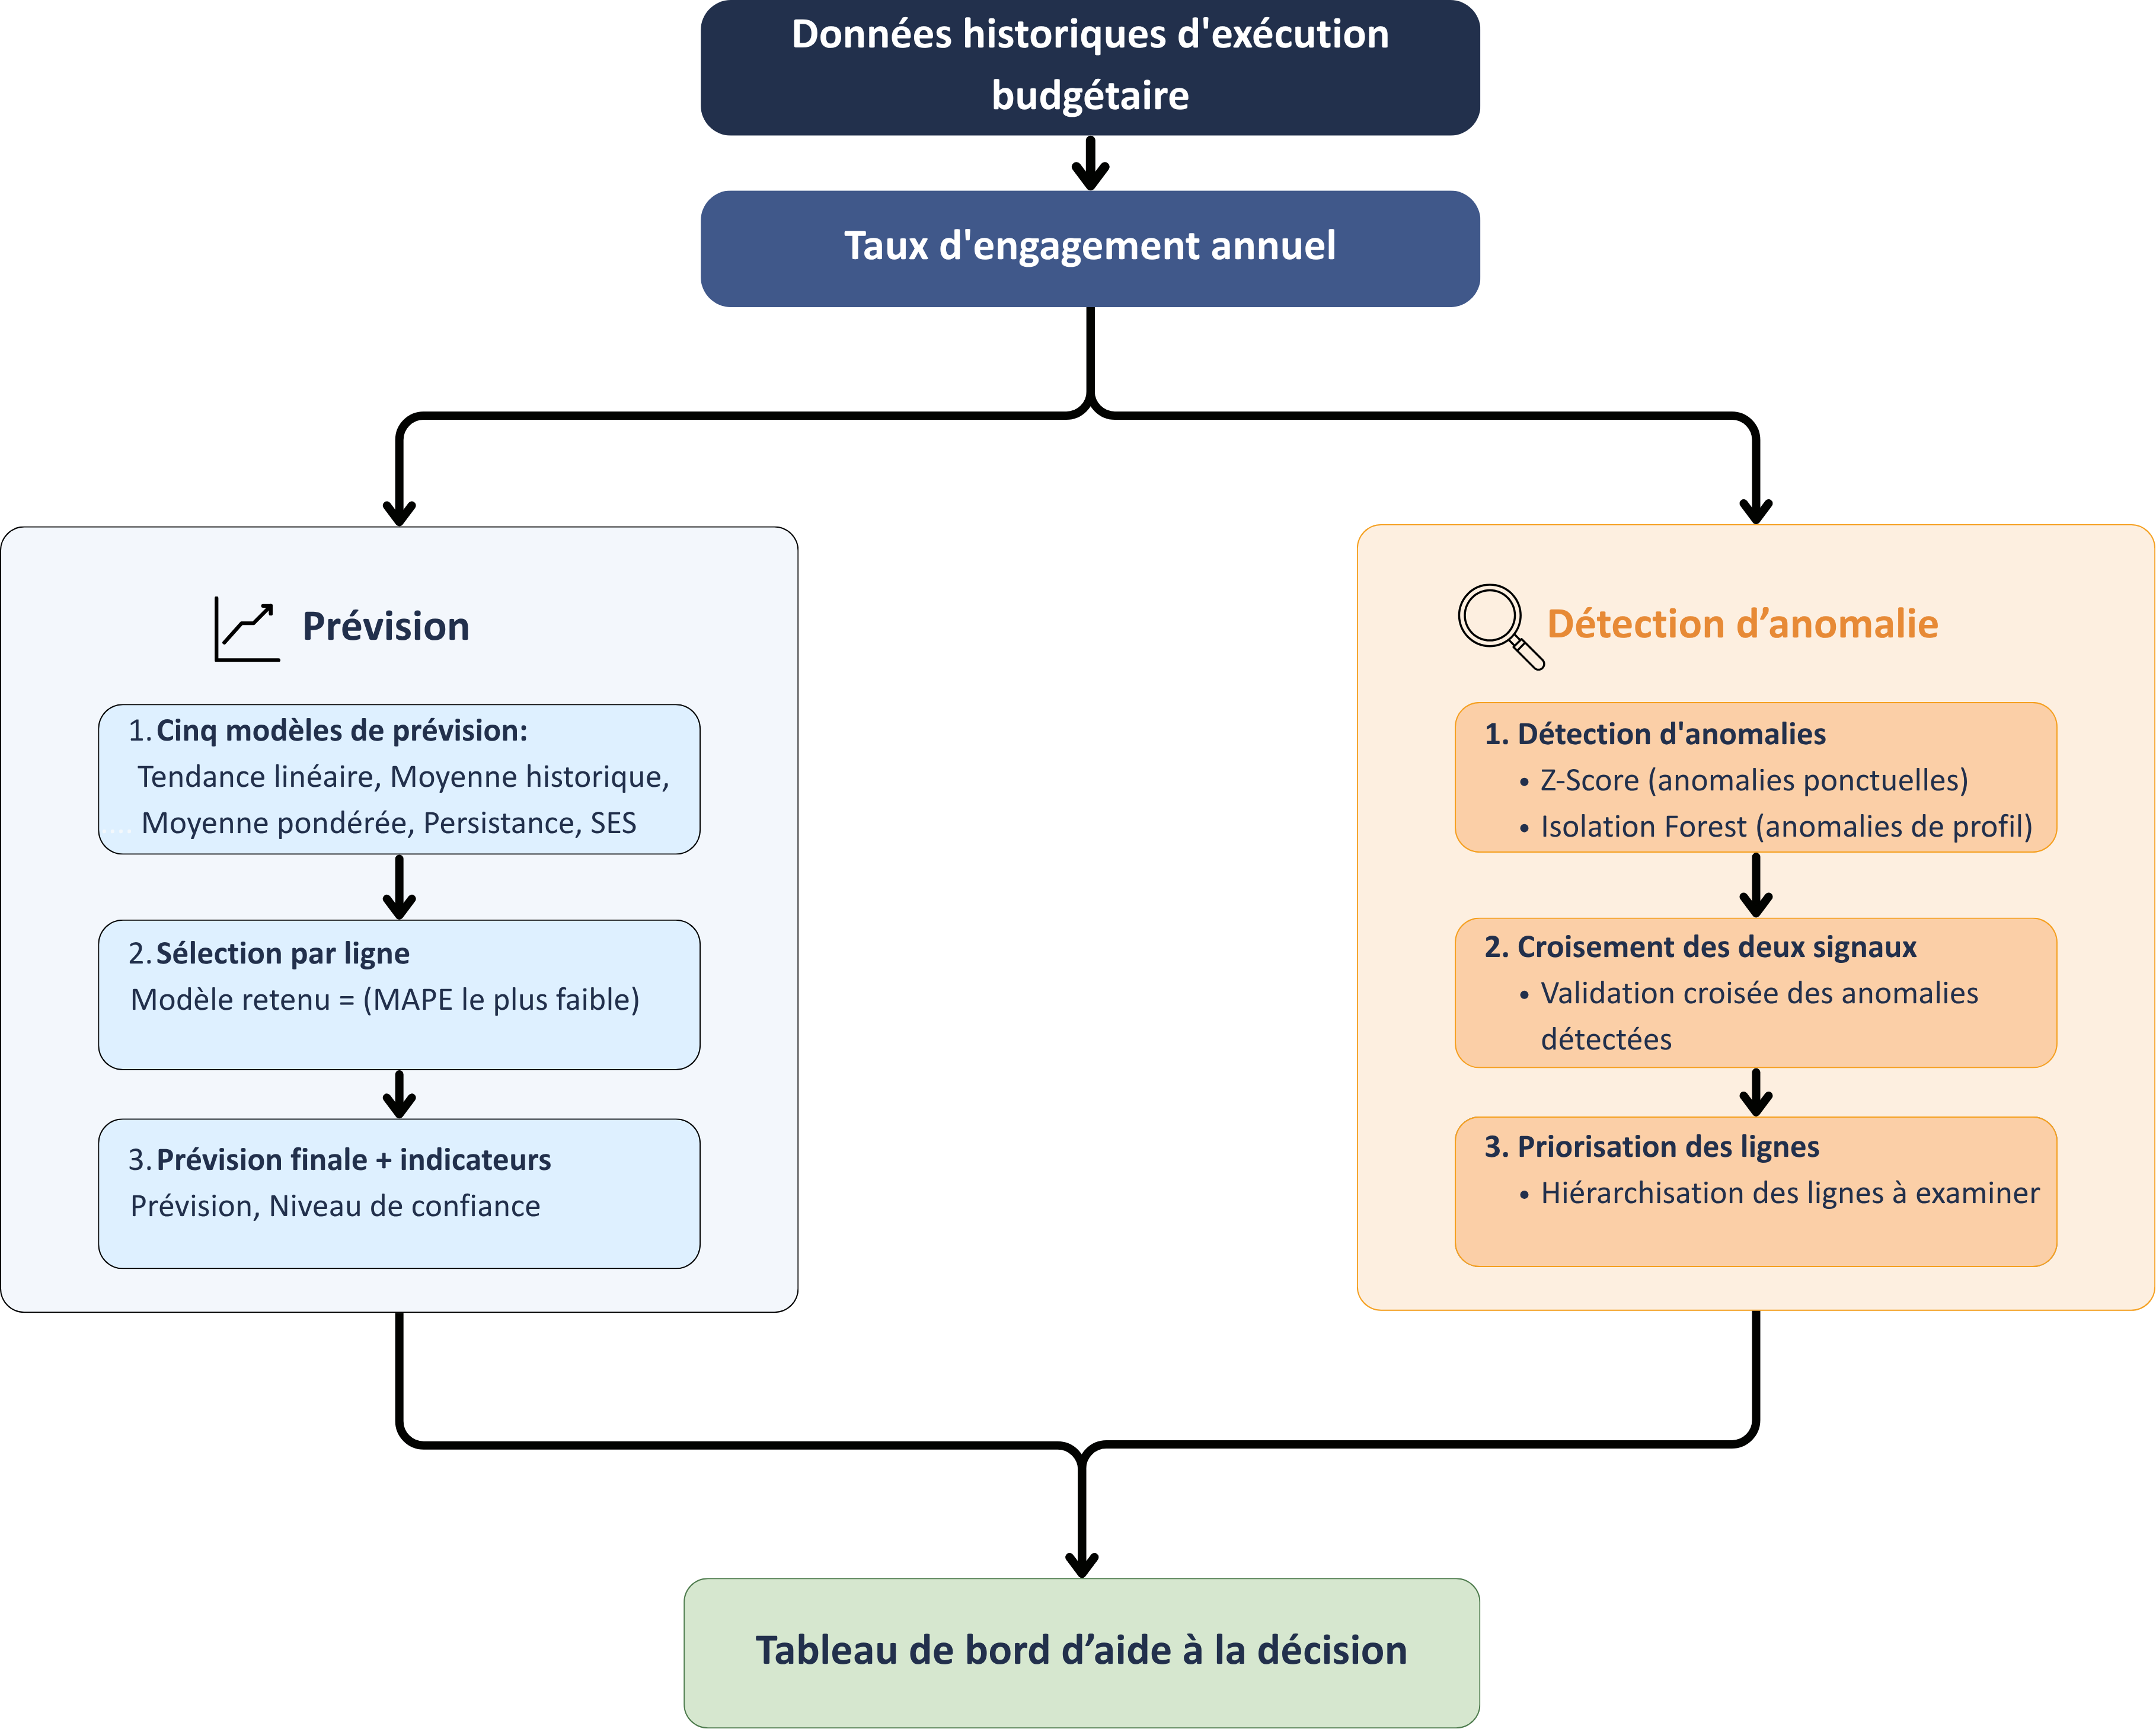
\includegraphics[width=0.7\textwidth]{figures/figure7.png}
\caption{Articulation g\'en\'erale du dispositif de pr\'evision et de
d\'etection d'anomalies pr\'esent\'e dans ce chapitre.}
\label{fig:pipeline-ch3}
\end{figure}

Cette repr\'esentation met en \'evidence le r\^ole compl\'ementaire des deux
branches~: la pr\'evision fournit une estimation chiffr\'ee assortie d'un
indicateur de confiance, tandis que la d\'etection d'anomalies oriente
l'attention du gestionnaire vers les lignes pr\'esentant des comportements
sp\'ecifiques. La combinaison de ces deux sorties au sein d'un m\^eme
livrable constitue la r\'eponse m\'ethodologique apport\'ee aux enjeux de
pilotage budg\'etaire identifi\'es au d\'ebut du chapitre.
